%-----------------------------------------------------------------------------%
\chapter{\babDua}
%-----------------------------------------------------------------------------%
%-----------------------------------------------------------------------------%
\section{Penelitian Sebelumnya}
%-----------------------------------------------------------------------------%
Penelitian-penelitian yang berhubungan dengan penelitian ini adalah penelitian mengenai convolutional neural network dan thin client pada teknologi mobile. Penelitian-penelitian tersebut memiliki keterhubungan seperti yang dapat dilihat pada \ref{fig:mind_map}.\\
\begin{figure}[htp]
	\centering
	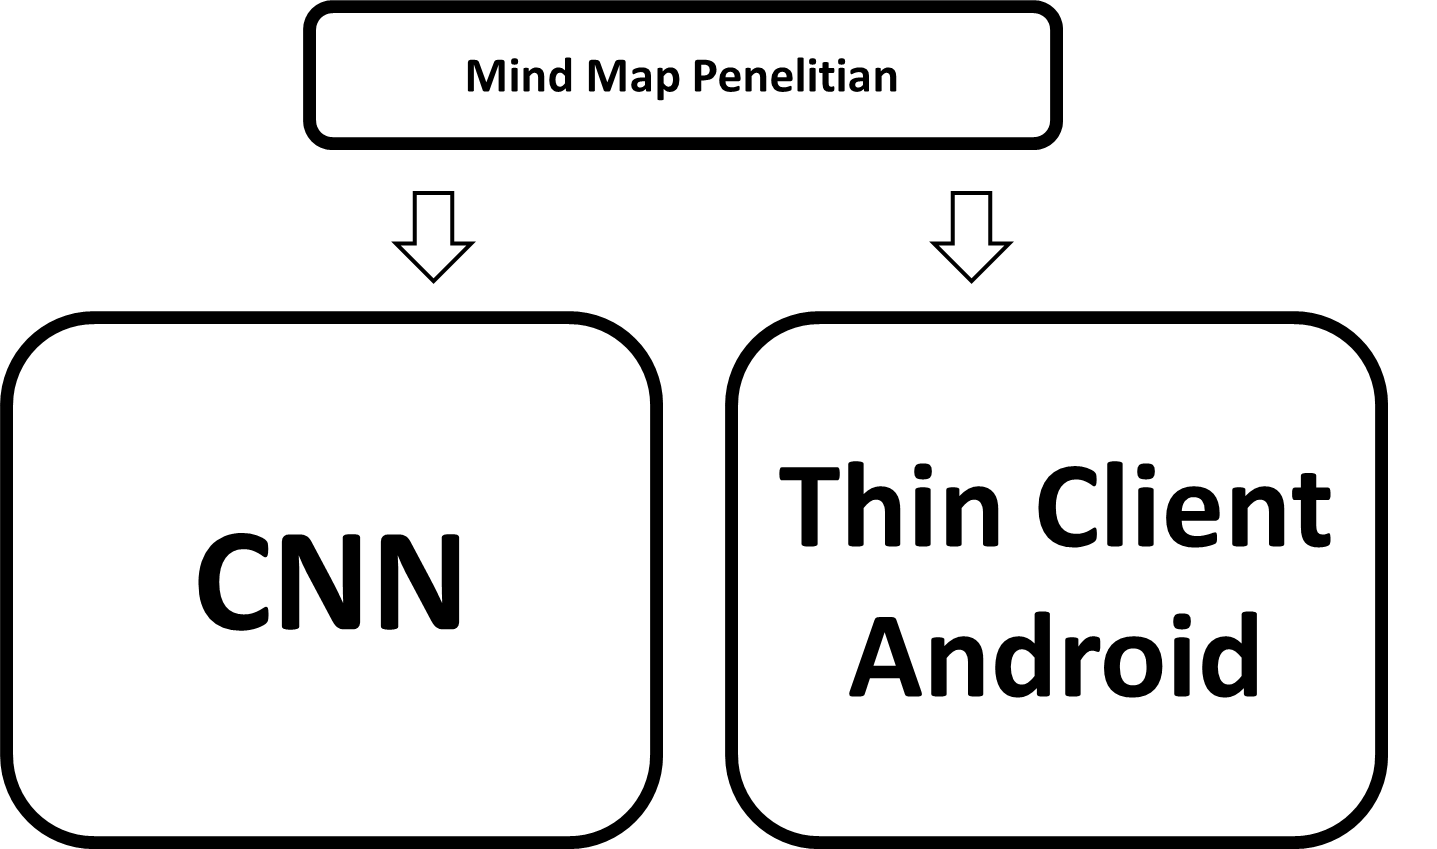
\includegraphics[width=8cm]{pics/mind_map_final}
	\caption{Mind map penelitian terdahulu terkait CNN}
	\label{fig:mind_map}
\end{figure}

Dalam penelitian \cite{can_deep_learning} yang dilakukan Nicholas D. LanePetko Georgiev, membangun prototipe deep neural network pada lingkungan low-power yang melibatkan CPU dan DSP dari perangkat mobile SoC (System On Chip). Deep Neural Network digunakan untuk melakukan deteksi aktivitas dan dilakukan perbandingan dengan teknik pembelajaran umum lainnya. Penelitian ini menemukan DNN mampu melakukan komputasi tanpa memberikan beban pada perangkat mobile dan mampu meningkatkan akurasi inferensi. Selain itu, ditemukan bahwa Deep Neural Network dapat dengan baik bekerja pada skala kelas inferensi yang lebih besar dan dipartisi secara fleksibel pada sumber daya perangkat mobile.

Dalam penelitian \cite{deepear} yang dilakukan oleh Nicholas Lane, Petko Georgiev dan Lorena Qendro, menyajikan DeepEar yang merupakan framework perangkat mobile audio pertama dengan metode Deep Neural Network pada sensor audio secara simultan. Penelitian ini membuktikan bahwa DeepEar layak digunakan pada perangkat mobile yang dibangun dengan cloud yang berjalan secara kontinyu dan menghabiskan sumber daya 6\% per hari.

Dalam penelitian \cite{early_Resource} yang dilakukan oleh Nicholas D. Lane, Sourav Bhattacharya, Petko Georgiev, Claudio Forlivesi dan Fahim Kawsar, meneliti perhitungan model deep learning (misalnya Convolutional Neural Network) pada perangkat mobile dan platform embedded. Penelitian ini bertujuan untuk mempelajari performa sistem, kebutuhan sumber daya dan bottleneck pada perangkat mobile ketika melakukan proses deep learning. Hasil dari penelitian ini memberikan fondasi untuk melakukan optimasi pada metode deep learning agar bisa diintegrasikan dengan teknologi IoT, smartphone dan sistem wearable.

Dalam penelitian \cite{deepx} yang dilakukan oleh Nicholas D. Lane, Sourav Bhattacharya, Petko Georgiev, Claudio Forlivesi, Lei Jiao, Lorena Qendro, dan Fahim Kawsar, menyajikan desain dan implementasi DeepX, yang merupakan perangkat lunak akselerator untuk melakukan proses deep learning. DeepX menyediakan algoritma untuk melakukan kontrol sumber daya ketika melakukan proses deep learning dengan melakukan dekomposisi model jaringan kedalam beberapa unit. Arsitektur DeepX membuktikan proses deep learning dapat melakukan proses secara efisien pada perangkat prosesor mobile modern.

Dalam penelitian \cite{smart_to_deep} yang dilakukan oleh Sourav Bhattacharya dan Nicholas D. Lane, meneliti metode Restricted Boltzmann Machines (RBM) untuk melakukan deteksi aktivitas pada perangkat smartwatch. Penelitian ini menyertakan variasi aktivitas seperti mode transportasi, aktivitas fisik dan deteksi lingkungan baik didalam ataupun diluar ruangan. Penelitian ini menunjukan Restricted Boltzmann Machines (RBM) dapat menggunakan sumber daya dengan efisien dan memungkinkan penggunaan deep learning pada perangkat smartwatch.

Dalam penelitian \cite{fast_rcnn} yang dilakukan oleh Ross Girshick, menciptakan metode deep learning Fast R-CNN yang merupakan penggabungan dari Region Convolutional Neural Network dan Spatial pyramid pooling networks (SPPnets). Penelitian ini bertujuan untuk memperbaiki kekurangan waktu komputasi R-CNN dan SPPnets pada saat training dan deteksi objek yang disebabkan multi-stage pipeline. Penelitian ini memberikan kontribusi perbaikan R-CNN dengan memberikan State-of-the-art mAP untuk VOC07, 2010, and 2012, waktu komputasi pembelajaran dan training yang lebih cepat dibandingkan R-CNN dan SPPnet dan fine-tune layer konvolusi.

Penelitian-penelitian terdahulu yang telah dijelaskan di atas dapat dituliskan dalam sebuah matriks literatur yang dapat dilihat pada tabel \ref{tab:tab1} sebagai berikut.
\begin{table}
	\clearpage
	\centering
	\caption{Matriks literatur penelitian terdahulu yang berhubungan dengan penelitian Convolution Neural Network}
	\label{tab:tab1}
	\begin{tabular}{ |m{2cm}|m{7cm}|m{1cm}|m{1cm}| } 	
		\hline	
		Judul & \multicolumn{3}{|m{13cm}|}{Can Deep Learning Revolutionize Mobile Sensing} \\
		\hline
		Pengarang & \multicolumn{3}{|m{13cm}|}{Nicholas D. Lane \& Petko Georgiev} \\ 
		\hline
		Tahun & \multicolumn{3}{|m{13cm}|}{2015} \\ 
		\hline
		Metode & \multicolumn{3}{|m{13cm}|}{Implementasi Deep Neural Network pada soc mobile dan DSP (Digital Signal Processor)}\\
		\hline
		Kontribusi  & \multicolumn{3}{|m{13cm}|}{Implementasi Deep Learning dengan memanfaatkan sensor pada mobile}\\ 
		\hline
		Pekerjaan Mendatang  & \multicolumn{3}{|m{13cm}|}{Pengembangan penggunaan sensor mobile dengan deep learning} \\
		\hline\hline
		Judul & \multicolumn{3}{|m{13cm}|}{DeepEar: Robust Smartphone Audio Sensing in Unconstrained Acoustic Environments using Deep Learning} \\
		\hline
		Pengarang & \multicolumn{3}{|m{13cm}|}{Nicholas D. Lane, Petko Georgiev, Lorena Qendro} \\ 
		\hline
		Tahun & \multicolumn{3}{|m{13cm}|}{2015} \\ 
		\hline
		Metode & \multicolumn{3}{|m{13cm}|}{Implementasi Deep Neural Network untuk sensor audio pada mobile}\\
		\hline
		Kontribusi  & \multicolumn{3}{|m{13cm}|}{Implementasi deep learning untuk sensor audio pada mobile dan arsitektur yang memberikan efisiensi pada konsumsi daya perangkat mobile}\\ 
		\hline
		Pekerjaan Mendatang  & \multicolumn{3}{|m{13cm}|}{Pengembangan sensor audio mobile untuk pengenalan aktivitas} \\
		\hline
		\hline\hline
		Judul & \multicolumn{3}{|m{13cm}|}{An Early Resource Characterization of Deep Learning on Wearables, Smartphones and Internet-of-Things Devices} \\
		\hline
		Pengarang & \multicolumn{3}{|m{13cm}|}{Nicholas D. Lane, Sourav Bhattacharya, Petko Georgiev, Claudio Forlivesi, Fahim Kawsar} \\ 
		\hline
		Tahun & \multicolumn{3}{|m{13cm}|}{2015} \\ 
		\hline
		Metode & \multicolumn{3}{|m{13cm}|}{Implementasi deep learning pada mobile dan platform embedded untuk meneliti performansi dan kebutuhan sumber daya mobile}\\
		\hline
		Kontribusi  & \multicolumn{3}{|m{13cm}|}{Memberikan pondasi penelitian metode deeplearning untuk teknologi IoT, smartphone and sistem wearable}\\ 
		\hline
		Pekerjaan Mendatang  & \multicolumn{3}{|m{13cm}|}{Pengembangan lanjut deeplearning pada teknologi IoT dan sistem wearable} \\
		\hline\hline
		Judul & \multicolumn{3}{|m{13cm}|}{DeepX: A Software Accelerator for Low-Power Deep Learning Inference on Mobile Devices} \\
		\hline
		Pengarang & \multicolumn{3}{|m{13cm}|}{Nicholas D. Lane, Sourav Bhattacharya, Petko Georgiev, Claudio Forlivesi, Lei Jiao, Lorena Qendro dan Fahim Kawsar} \\ 
		\hline
		Tahun & \multicolumn{3}{|m{13cm}|}{2016} \\ 
		\hline
		Metode & \multicolumn{3}{|m{13cm}|}{Dekomposisi model arsitektur deep learning menjadi beberapa blok unit dan pengaturan sumber daya model deep learning}\\
		\hline
	\end{tabular}
\end{table}

\begin{table}
	\clearpage
	\centering
	\begin{tabular}{ |m{2cm}|m{7cm}|m{1cm}|m{1cm}| } 	
		\hline
		Kontribusi  & \multicolumn{3}{|m{13cm}|}{Optimasi sumber daya model deep learning untuk mobile}\\ 
		\hline
		Pekerjaan Mendatang  & \multicolumn{3}{|m{13cm}|}{Implementasi arsitektur DeepX pada mobile dengan variasi metode deep learning} \\
		\hline\hline	
		Judul & \multicolumn{3}{|m{13cm}|}{Fast R-CNN} \\
		\hline
		Pengarang & \multicolumn{3}{|m{13cm}|}{Ross Girshick} \\ 
		\hline
		Tahun & \multicolumn{3}{|m{13cm}|}{2015} \\ 
		\hline
		Metode & \multicolumn{3}{|m{13cm}|}{Integrasi dan optimasi Region-CNN dan Spatial pyramid pooling networks}\\
		\hline
		Kontribusi  & \multicolumn{3}{|m{13cm}|}{Optimasi Region-CNN dan Spatial pyramid pooling networks}\\ 
		\hline
		Pekerjaan Mendatang  & \multicolumn{3}{|m{13cm}|}{Peningkatan deteksi objek dengan perbaikan metode sparse object} \\
		\hline
	\end{tabular}
\end{table}
%-----------------------------------------------------------------------------%
\section{\f{Feedforward Neural Network}} \label{fnn}
%-----------------------------------------------------------------------------%
Di dalam \f{machine learning}, \f{artificial neural network} (ANN) adalah model yang terinspirasi oleh \f{neural network} biologis. \f{Aritificial neural network} dapat melakukan estimasi atau aproksimasi fungsi non-linear dengan nilai \f{output} yang dapat berupa nilai \f{real}, diskret, atau vektor. Pada alamnya, neuron menerima sinyal melalui sinaps yang terletak pada dendrit. Neuron akan teraktivasi dan dapat meneruskan sinyal apabila sinyal yang diterima memenuhi batas tertentu. Sinyal tersebut dapat diterima sinaps lain dan dapat mengaktivasi neuron lainnya. Beberapa permasalahan yang dapat diselesaikan dengan ANN diantaranya adalah klasifikasi, kategorisasi, aproksimasi fungsi, dan prediksi .

\f{Feedforward neural network} adalah salah satu jenis ANN. \f{Feedforward neural network} terdiri dari beberapa unit yang dikelompokkan dalam \f{layer} di mana setiap \f{layer} yang bersebelahan saling terhubung melalui suatu unit. Pada \f{feedforward neural network}, koneksi antar \f{unit} tidak membentuk \f{cycle} seperti yang ada pada \f{recurrent neural network}. Kalkulasi \f{feedforward neural network} dari \f{input} ke \f{output} berjalan ke satu arah sesuai dengan strukturnya yang tampak seperti graf berarah. Contoh \f{feedforward neural network} dengan satu \f{hidden layer} dapat dilihat pada Gambar \ref{fig:fnn} berikut.

\begin{figure}
	\centering
	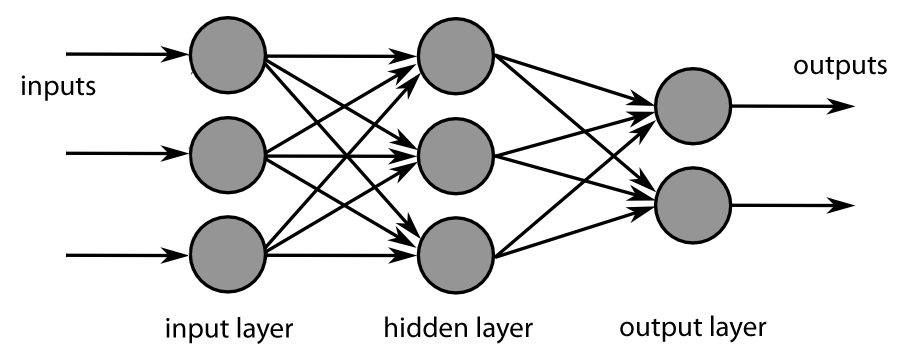
\includegraphics[width=0.8\textwidth,height=0.3\textwidth]
	{pics/fnn.png}
	\caption{Contoh \f{feedforward neural network}}
	\label{fig:fnn}
\end{figure}
\vspace{-1.2cm}
\begin{center}
	{\small Sumber gambar: http://technobium.com/stock-market-prediction-using-neuroph-neural-networks/}
\end{center}

\f{Feedforward neural network} terdiri dari \f{input layer}, \f{output layer}, dan beberapa \f{hidden layer} apabila dibutuhkan. Jumlah \f{hidden layer} berperan pada seberapa kompleks batas keputusan yang dapat dibentuk oleh \f{network} seperti pada Gambar \ref{fig:hl}.

\begin{figure}
	\centering
	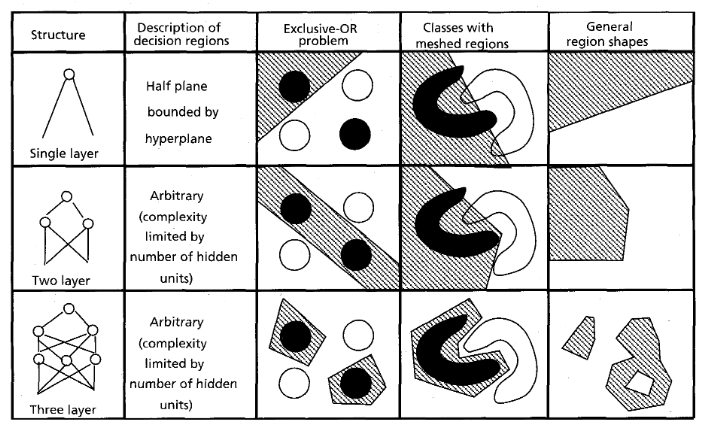
\includegraphics[width=1\textwidth,height=0.6\textwidth]
	{pics/hl.png}
	\caption{Interpretasi geometris pada peran \f{hidden layer}}
	\label{fig:hl}
\end{figure}
\vspace{-1.2cm}
\begin{center}
	{\small Sumber gambar: \cite{jain}}
\end{center}

Pada \f{input layer}, jumlah unit atau neuron yang ada sesuai dengan jumlah elemen yang ada pada vektor \f{input}. Begitu juga dengan \f{output layer}, jumlah unit yang ada sesuai dengan banyaknya elemen yang diinginkan pada vektor \f{output}. Berbeda dengan \f{input layer} dan \f{output layer}, jumlah unit dalam \f{hidden layer} sifatnya bebas. Setiap unit menghasilkan suatu \f{output} dari kombinasi linear beberapa nilai \f{input} dengan bobotnya masing-masing. Hasil dari kombinasi linear tersebut kemudian diaktivasi dengan fungsi aktivasi. Proses ini dapat dilihat pada Rumus \ref{equ:perceptron}.

\begin{equation}
\label{equ:perceptron}
y(x) = g\left(\sum\limits_{i=1}^{n} w_{ij}x_{i} + w_{0j}\right)
\end{equation}

\begin{itemize}
	\item $x$ merupakan vektor \f{input}
	\item $w$ merupakan vektor bobot
	\item $w_{ij}$ merupakan bobot yang menghubungkan unit ke-\f{i} pada \f{layer} sebelumnya dan unit ke-\f{j} pada \f{layer} saat itu
	\item $w_{0j}$ merupakan bobot untuk bias
	\item $g$ merupakan fungsi aktivasi
\end{itemize}

Pada Rumus \ref{equ:perceptron} vektor \f{input} pada suatu \f{layer} bergantung pada \f{output} di \f{layer} sebelumnya, kecuali untuk \f{layer} pertama yaitu \f{input layer}. Fungsi aktivasi $g$ dapat berbeda untuk setiap \f{layer}, tapi pada umumnya sama untuk setiap unit pada \f{layer} yang sama. Pada penelitian ini fungsi aktivasi yang digunakan adalah \f{rectified linear unit} (ReLU) yang dapat dilihat pada Rumus \ref{equ:relu}, dan \f{sigmoid} pada Rumus \ref{equ:sigmoid}.

\begin{equation}
\label{equ:relu}
g(x) = max(0, x)
\end{equation}

\begin{equation}
\label{equ:sigmoid}
g(x) = \frac{1}{1 + e^{-x}}
\end{equation}

Pada Rumus \ref{equ:perceptron} terdapat $w_{0j}$ yang merupakan bobot untuk bias. Bias bersifat seperti konstanta yang selalu bernilai +1, sehingga pengaruh bias tergantung pada bobotnya.

%-----------------------------------------------------------------------------%
\section{Convolution Neural Network (CNN)}
%-----------------------------------------------------------------------------%
CNN merupakan salah satu variasi dari multilayer perceptron (MLP). Keuntungan dari metode CNN, khsusnya untuk kasus pengenalan pola dibandingkan pendekatan konvensional adalah kemampuan untuk mengurangi dimensi data, ekstraksi fitur secara sekuensial, dan mengklasifikasi salah satu struktur jaringan. Arsitektur dasar dari model CNN terinspirasi dari visual cortex yang dikenalkan oleh hubel dan wiesel pada tahun 1962.

Pada tahun 1980, neocognitron fukushima membuat pertama kali komputasi menggunakan model CNN, dan kemudian pada tahun 1989, dengan menggunakan model yang ditemukan fukushima, LeCun menemukan performa dari beberapa proses untuk pengenalan pola menggunakan metode error gradient.

Model CNN yang digunakan oleh LeCun merupakan pengembangan dari MLP tradisional yang didasari 3 ide, local receptive field, weight sharing dan spatial subsampling. Ide dasar ini diorganisir kedalam 2 tipe layer, yaitu convolution dan subsampling layer. Seperti yang ditunjukan gambar 1, digunakan 3 convolution layer dengan kombinasi layer subsampling dan 1 output layer. Layer convolution dan subsampling tersusun kedalam plane atau disebut feature maps.

\f{Convolutional neural network} (CNN) adalah salah satu tipe \f{feedforward neural network} yang terinspirasi dari cara kerja visual korteks. Berdasarkan penelitian \cite{hubel_weasel}, korteks visual terdiri dari banyak sel kompleks. Sel-sel ini disebut \f{receptive field} dan sensitif terhadap bagian kecil bidang visual. Salah satu sifat yang dimiliki CNN adalah \f{sparse connectivity}. \f{Sparse connectivity} memungkinkan suatu \f{layer} saling terhubung hanya dengan unit-unit terdekat. Dengan kata lain, \f{input} dari suatu unit merupakan \f{subset} dari unit pada \f{layer} sebelumnya. Ilustrasi \f{sparse connectivity} dapat dilihat pada Gambar.

\begin{figure}
	\centering
	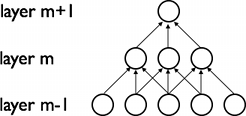
\includegraphics[width=0.45\textwidth,height=0.2\textwidth]
	{pics/sparse.png}
	\caption{\f{Sparse Connectivity}}
	\label{fig:sparse}
\end{figure}
\vspace{-1.2cm}
\begin{center}
	{\small Sumber gambar: http://deeplearning.net/tutorial/lenet.html}
\end{center}

Tumpukan \f{layer} pada Gambar \ref{fig:sparse} hanya memiliki satu unit pada \f{layer} $m + 1$. Hal ini merepresentasikan unit atau bagian-bagian kecil yang ada pada \f{layer} $m - 1$ bagaikan disaring atau di-\f{filter} hingga \f{layer} $m + 1$ memahami bidang visual secara utuh. 

Selain \f{sparse connectivity}, CNN juga memiliki sifat \f{shared weights}. Setiap \f{layer} kecuali \f{output layer} memiliki \f{filter} yang fungsinya untuk menyaring bagian kecil dari bidang visual. \f{Filter} tersebut direplikasi dengan bobot yang sama ke seluruh bidang visual dengan untuk menyaring unit atau bagian-bagian kecil sehingga membentuk \f{feature map}. Pada Gambar \ref{fig:shared} berikut, lima unit pada \f{layer} $m - 1$ disaring dengan \f{filter} berukuran tiga, sehingga membentuk tiga unit \f{feature map}. Garis yang berwarna sama menandakan bobot yang sama.

\begin{figure}
	\centering
	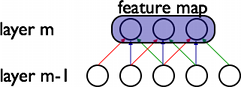
\includegraphics[width=0.45\textwidth,height=0.15\textwidth]
	{pics/shared.png}
	\caption{\f{Shared weights} untuk \f{filter} yang sama}
	\label{fig:shared}
\end{figure}
\vspace{-1.2cm}
\begin{center}
	{\small Sumber gambar: http://deeplearning.net/tutorial/lenet.html}
\end{center}

Untuk merepresentasikan data atau bidang visual yang kompleks, setiap \f{layer} pada CNN dapat mempunyai beberapa \f{feature map} atau \f{channel}. Rumus untuk menghitung \f{feature map} ke-$k$ pada \f{pixel} koordinat $(i,j)$ yang ditentukan oleh bobot $W^{k}$ dan bias $b_{k}$ adalah sebagai berikut.

\begin{equation}
\label{equ:featuremap}
y^{k}_{ij} = g\left((W^{k} * x)_{ij} + b_{k}\right)
\end{equation}

Setiap \f{feature map} pada layer $m - 1$ berkontribusi dalam menentukan nilai \f{feature map} $k$ pada layer $m$. Dengan kata lain, setiap \f{pixel} yang berada dalam \f{feature map} $k$ nilainya akan ditentukan oleh seluruh \f{pixel} yang terhubung, pada \f{feature map} di \f{layer} $m - 1$. Pada ilustrasi Gambar \ref{fig:featuremap}, \f{layer} $m$ memiliki dua \f{feature map} $y^0$ dan $y^1$. \f{Pixel} (kotak berwarna biru) pada $y^0$ ditentukan dari 2x2 \f{pixel} yang terhubung dengan bobot $W^{kl}_{ij}$. $W^{kl}_{ij}$ menyatakan bobot yang menghubungkan \f{pixel} koordinat $(i,j)$ pada \f{feature map} ke-$l$ di \f{layer} $m - 1$ ke \f{pixel} yang terhubung pada \f{feature map} ke-$k$ di \f{layer} $m$.

\begin{figure}
	\centering
	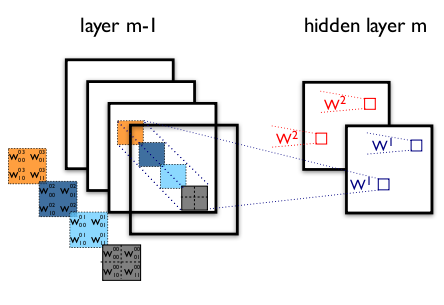
\includegraphics[width=0.9\textwidth,height=0.55\textwidth]
	{pics/featuremap.png}
	\caption{Ilustrasi \f{layer} pada \f{convolutional neural network}}
	\label{fig:featuremap}
\end{figure}
\vspace{-1.2cm}
\begin{center}
	{\small Sumber gambar: http://deeplearning.net/tutorial/lenet.html}
\end{center}

\f{Convolutional Neural Network} biasanya terdiri dari beberapa \f{filter} atau disebut juga dengan \f{convolutional layer}, sering kali diikuti denga \f{subsampling layer} dan diakhiri dengan \f{fully connected layers}. Terdapat juga jenis CNN yang tidak diakhiri dengan \f{fully connected layers} melainkan \f{convolutional layer} lainnya yang mempertahankan dimensi data dalam bentuk citra 2D. CNN jenis ini disebut dengan \f{Fully Convolutional Neural Network}.

\subsection{Convolutional Layer}
Pada layer convolution, tiap neuron terhubung secara local kepada area yang lebih kecil (local receptive field) pada layer sebelumnya. Semua neuron yang memiliki feature maps yang sama memperoleh data dari input area yang berbeda hingga semua input plan tersaring tetapi saling berbagi bobot (weight sharing).\\

\f{Convolutional layer} memiliki tiga \f{hyperparameter} yang mengatur transformasi \f{feature map} yang dihasilkan: \f{depth} $D$, \f{stride} $S$, dan \f{zero-padding} $P$. Dalam tahap \f{feedforward}, \f{convolutional layer} berukuran $F$ akan bergeser pada gambar berukuran $W$, dan menghasilkan \f{feature map} sebanyak $D$ dengan ukuran $W'$ yang dapat dihitung menggunakan Rumus \ref{equ:convlayer} berikut.

\begin{equation}
\label{equ:convlayer}
W' = (W - F + 2P) / S + 1
\end{equation}

Dalam praktiknya, \f{zero-padding} sering kali digunakan untuk menyesuaikan ukuran hasil \f{feature map}. \f{Zero padding} dengan ukuran $P = (F - 1)/2$ dipastikan menghasilkan \f{feature map} dengan ukuran yang sama dengan \f{feature map} sebelumnya apabila \f{stride} $S = 1$. \f{Deep learning framework} seperti \f{theano} menyebut \f{padding} dengan sifat tersebut sebagai \f{same padding} . Terdapat juga \f{full padding} yang menghasilkan \f{feature map} dengan ukuran $W' = W + F - 1$.

\subsection{Subsampling Layer}
Pada layer subsampling, feature maps didownsampling secara spasial, dimana ukuran map dikurangi berdasarkan 2 faktor. Contohnya, feature map pada layer C3 dengan ukuran 10x10 dilakukan subsampling untuk menyesuaikan feature map dengan ukuran 5x5 pada layer selanjutnya. Layer terakhir adalah F6 yang merupakan proses klasifikasi.
Dalam arsitektur \f{convolutional neural network}, \f{pooling layer} berfungsi untuk mereduksi ukuran spasial gambar secara bertahap sehingga mengurangi parameter dan komputasi pada \f{network}. \f{Pooling layer} menerima \f{input} \f{feature map} berukuran $W_{1}$ sebanyak $D_{1}$ dan parameter ukuran \f{pooling} $F$ dan \f{stride} $S$. Sama halnya dengan \f{convolutional layer}, \f{pooling layer} juga bergeser terhadap input dan menghasilkan \f{feature map} berjumlah $D_{2} = D_{1}$ dengan ukuran $W_{2} = (W_{1} - F)/S + 1$. Terdapat beberapa jenis \f{pooling layer}, dan yang paling sering digunakan adalah:

\begin{enumerate}
	\item \f{Max Pooling} \\
	Dalam \f{pooling} berukuran $F$, \f{Max pooling} akan mengambil hasil aktivasi yang terbesar dalam daerah yang termasuk pada pergeseran saat itu. Ilustrasi ini dapat dilihat pada Gambar \ref{fig:maxpool} berikut dengan $F = 2$ dan $S = 2$.
	
	\begin{figure}
		\centering
		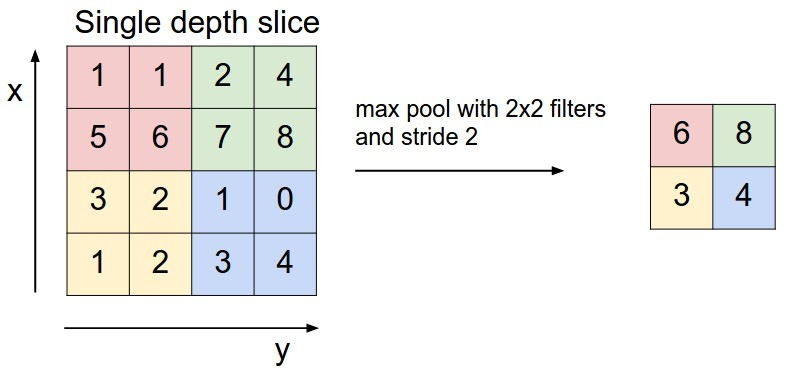
\includegraphics[width=0.8\textwidth,height=0.35\textwidth]
		{pics/maxpool.jpeg}
		\caption{Ilustrasi \f{max pooling}}
		\label{fig:maxpool}
	\end{figure}
	\vspace{-1.2cm}
	\begin{center}
		{\small Sumber gambar: http://cs231n.github.io/convolutional-networks}
	\end{center}
	
	\item \f{Average Pooling} \\
	Berbeda dengan \f{max pooling}, \f{average pooling} mengambil hasil aktivasi pada daerah \f{filter} dan menghitung rata-rata dari seluruh hasil aktivasi dalam daerah tersebut.
\end{enumerate}
%-----------------------------------------------------------------------------%
\subsection{\f{Fully Connected Layer}}
%-----------------------------------------------------------------------------%
\f{Fully connected layer} adalah \f{feed forward neural network} yang dijelaskan pada subbab \ref{fnn}. Biasanya, \f{fully connected layer} berada pada \f{layer} akhir pada arsitektur \f{convolutional neural network} dan bertujuan untuk memproses hasil \f{feature extraction} yang dilakukan pada \f{layer} sebelumnya menjadi suatu \f{output} tertentu. Gambar \ref{fig:cnnlayers} berikut merupakan contoh arsitektur dengan susunan \f{convolutional layer}, \f{pooling layer}, dan \f{fully connected layer}.

\begin{figure}
	\centering
	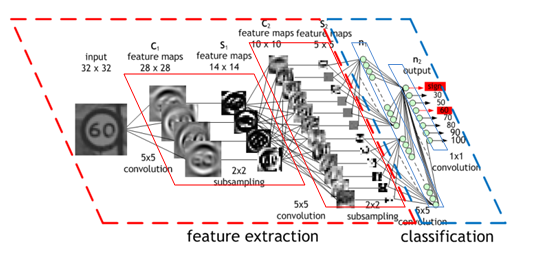
\includegraphics[width=1\textwidth,height=0.45\textwidth]
	{pics/cnnlayers.png}
	\caption{Contoh arsitektur \f{convolutional neural network}}
	\label{fig:cnnlayers}
\end{figure}
\vspace{-1.2cm}
\begin{center}
	{\small Sumber gambar: https://devblogs.nvidia.com}
\end{center}
%-----------------------------------------------------------------------------%
\section{\f{Backpropagation}}
%-----------------------------------------------------------------------------%
Tujuan dari melatih model \f{feedforward neural network} adalah membuat model tersebut dapat memprediksi nilai dengan galat seminimal mungkin. \f{Feedforward neural network} menggunakan metode \f{backpropagation} untuk melatih nilai bobot-bobot pada \f{network} tersebut. Untuk melatih suatu bobot, metode ini melakukan \f{propagation} dari galat pada \f{output layer} sehingga informasi ini tersebar ke \f{layer} sebelumnya untuk digunakan dalam mengubah bobot.

Untuk $\delta^{(l+1)}$ sebagai galat pada \f{layer} $l+1$ dengan fungsi galat $J(W,b;x,y)$ di mana $W,b$ adalah parameter, dan $x,y$ adalah pasangan \f{input} dan label, apabila \f{layer} $l$ dan \f{layer} $l+1$ saling terhubung maka galat pada \f{layer} $l$ adalah sebagai berikut.


\begin{equation}
\begin{aligned}
\delta^{(l)} &= ((W^{(l)})^{T}\delta^{(l+1)}) \cdot f'(z^{(l)}) \\
f'(z^{(l)}) &= a^{(l)} \cdot (1-a^{(l)})
\end{aligned}
\end{equation}

\begin{equation}
\label{equ:erder}
\begin{aligned}
\Delta_{w^{(l)}}J(W,b;x,y)&=\delta^{(l+1)}(a^{(l)})^{T} \\
\Delta_{b^{(l)}}J(W,b;x,y)&=\delta^{(l+1)}
\end{aligned}
\end{equation}

Pada \f{convolutional layer} dan \f{pooling layer}, galat pada \f{layer} $l$ dihitung dengan fungsi \f{upsample} $g(x)$ tergantung pada \f{layer} yang digunakan.

\begin{equation}
\label{equ:errorc}
\delta^{(l)}_{k} = upsample((W^{(l)}_{k})^{T}\delta^{(l+1)}_{k}) \cdot f'(z^{(l)}_{k}) 
\end{equation}

\[
g(x)
\begin{cases}
\frac{\sum_{k=1}^{m} x_{k}}{m}, \frac{\delta g}{\delta x} = \frac{1}{m}, & \text{average pooling} \\
max(x), \frac{\delta g}{\delta x} =
\begin{cases}
1, & \text{if } x_{i} = max(x) \\
0, & otherwise
\end{cases}
, & \text{max pooling}
\end{cases}
\]

\begin{center}
	{\small Sumber rumus: http://www.slideshare.net/kuwajima/cnnbp}
\end{center}

Rumus \ref{equ:erder} digunakan untuk mengubah bobot pada suatu \f{layer}. Salah satu cara untuk mengubah bobotnya adalah dengan \f{stochastic gradient descent} yang menggunakan Rumus \ref{equ:sgd} berikut.

\begin{equation}
\label{equ:sgd}
\theta = \theta-\alpha\Delta_{\theta}J(\theta;x^{(i)},y^{(i)})
\end{equation}

\begin{center}
	{\small Sumber rumus: http://ufldl.stanford.edu/tutorial/supervised/ConvolutionalNeuralNetwork}
\end{center}


%-----------------------------------------------------------------------------%
\section{Algoritma Optimasi}
%-----------------------------------------------------------------------------%
Algoritma optimasi digunakan untuk permasalahan meminimalisasi \f{loss}. Untuk \f{dataset} $D$, objektif dari optimasi adalah rata-rata $loss$ $|D|$ dari seluruh anggota \f{dataset} $D$. Dengan $fw(X^{(i)})$ adalah galat pada data ke $X^{(i)}$, dan $r(W)$ adalah regularisasi dengan bobot $\lambda$, maka galat rata-rata dapat dihitung menggunakan Rumus \ref{equ:avgloss} berikut .

\begin{equation}
\label{equ:avgloss}
L(W)=\frac{1}{|D|}\sum\limits_{i}^{|D|}fw(X^{(i)})+\lambda r(W)
\end{equation}

Karena $|D|$ pada kenyataannya dapat bernilai sangat besar, dalam praktiknya setiap iterasi menggunakan aproksimasi secara stokastik dengan memilih $N << |D|$ sehingga galat rata-rata dihitung dengan Rumus \ref{equ:avgloss2} berikut .

\begin{equation}
\label{equ:avgloss2}
L(W)\approx\frac{1}{N}\sum\limits_{i}^{N}fw(X^{(i)})+\lambda r(W)
\end{equation}
%-----------------------------------------------------------------------------%
\subsection{\f{Stochastic Gradient Descent} (SGD)}
%-----------------------------------------------------------------------------%
\f{Stochastic gradient descent} mengubah bobot $W$ dengan kombinasi linear dari \f{gradient} negatif $\Delta L(W)$ dan perbaharuan bobot $V_{t}$ pada iterasi sebelumnya. Untuk menghitung nilai perbaharuan $V_{t+1}$ dan bobot $W_{t+1}$ pada iterasi $t+1$ digunakan Rumus \ref{equ:sgd2} dan \ref{equ:sgd2-3} berikut .

\begin{equation}
\label{equ:sgd2}
V_{t+1} = \mu V_{t} - \alpha \Delta L(W_{t})
\end{equation}

\begin{equation}
\label{equ:sgd2-3}
W_{t+1} = W_{t} + V_{t+1}
\end{equation}
%-----------------------------------------------------------------------------%
\subsection{\f{Nesterov's Accelerated Gradient} (Nesterov)}
%-----------------------------------------------------------------------------%
\f{Nesterov's accelerated gradient} (Nesterov) diusulkan oleh Nesterov sebagai metode optimal untuk optimasi, dengan laju konvergensi mencapai $O(1/t^{2})$. Dalam praktiknya, Nesterov dapat menjadi metode yang cukup efektif untuk mengoptimasi arsitektur \f{deep learning} tertentu, seperti yang didemonstrasikan oleh  dalam membuat \f{autoencoders}. Perubahan bobot dalam algoritma Nesterov menggunakan Rumus berikut .

\begin{equation}
\label{equ:nesterov}
V_{t+1}=\mu V_{t} - \alpha\Delta L(W_{t} + \mu V_{t})
\end{equation}

\begin{equation}
W_{t+1} = W_{t} + V_{t+1}
\end{equation}

Perbedaan Nesterov dengan SGD terdapat pada penambahan momentum dalam menghitung \f{gradient} $\Delta L(W_{t} + \mu V_{t})$. Dalam SGD, perhitungan \f{gradient} $\Delta L(W_{t})$ hanya mengambil bobotnya saja.

%-----------------------------------------------------------------------------%
\section{Fungsi Galat}
%-----------------------------------------------------------------------------%
Fungsi galat adalah fungsi yang menghitung galat dari hasil prediksi $\hat{y}$ dengan nilai $y$ yang sebenarnya. Beberapa jenis fungsi galat, yaitu \f{cross-entropy loss} (Rumus \ref{equ:cl}) dan \f{euclidean loss} (L2) (Rumus \ref{equ:el}). Dilihat dari fungsinya, \f{cross entropy} bekerja lebih agresif dalam memperbaiki dibandingkan dengan \f{euclidean error}.

\begin{equation}
\label{equ:cl}
crossentropy(y, \hat{y}) = -(y * log(\hat{y}) + (1 - y) * log(1 - \hat{y}))
\end{equation}

\begin{equation}
\label{equ:el}
euclideanloss(y, \hat{y}) = \frac{1}{2} \|y - \hat{y}\|^{2}_{2}
\end{equation}
\begin{center}
	{\small Sumber rumus: http://caffe.berkeleyvision.org}
\end{center}
%-----------------------------------------------------------------------------%
\section{Fast R-CNN}
%-----------------------------------------------------------------------------%

Arsitektur Fast R-CNN \ref{fig:arsitektur_fcnn} memiliki input objek gambar dan gambar yang sudah diberikan RoI (Object Proposal). Input akan diproses pertama kali kedalam beberapa layer konvolusi dan max pooling untuk mendapatkan feature map. Kemudian tiap objek proposal dengan Region of Interest (RoI) akan melakukan ekstraksi fitur dari feature map. Tiap vektor dari fitur akan diproses secara berurutan kedalam Fully Connected Layer dan dipecah ke dalam 2 output layer. Layer pertama menggunakan probabilitas softmax untuk melakukan estimasi pada K kelas object dan background. Layer kedua memberikan 4 output dalam bentuk bilangan real untuk tiap K kelas objek. Untuk setiap 4 nilai dilakukan encoding posisi bounding-box pada salah satu posisi dari kelas K.

\begin{figure}[htp]
	\centering
	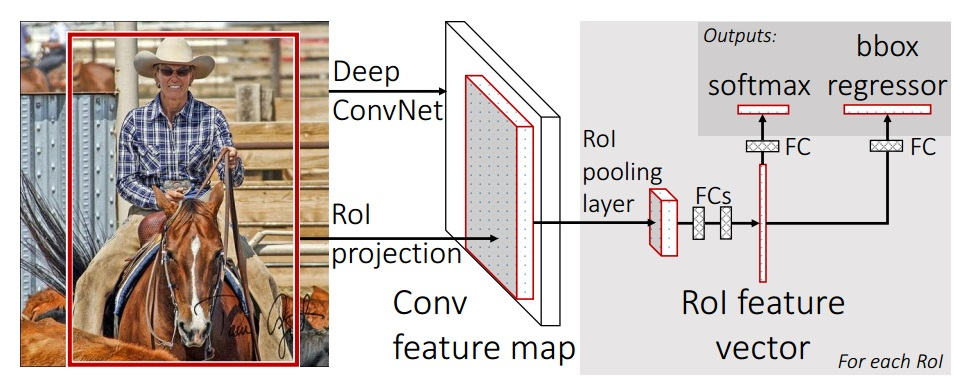
\includegraphics[width=10cm]{pics/arsitektur_fcnn}
	\caption{Arsitektur Fast R-CNN}
	\label{fig:arsitektur_fcnn}
\end{figure}

\subsection{RoI pooling layer}
RoI merupakan suatu area yang berbentuk segi empat dan berada didalam feature map konvolusi. Layer RoI pooling bertujuan melakukan proses max pooling dengan tujuan konversi fitur didalam RoI kedalam feature map yang lebih kecil dengan ukuran yang sudah didefinisikan sebelumnya. RoI didefinisikan menggunakan 4 tuple \f{(r, c, h, w)} dimana \f{(r, c)} mendefinisikan \f{top-left corner} dan \f{(h, w)} mendefinisikan nilai tinggi dan lebar.

Proses max poling pada RoI membagi area dengan \f{h x w} menjadi \f{H x W} sub-window dengan rumus \f{h/H x w/W}. Nilai sub-window tersebut akan memiliki korespondensi dengan output grid cell. Pooling dilakukan secara independen kepada tiap channel feature map yang merupakan standard dari max pooling.

\subsection{Pre-trained networks}
Pada penelitian \cite{fast_rcnn}, pra pembelajaran jaringan menggunakan 5 layer max pooling dan layer konvolusi dengan jumlah antara 5 hingga 13 layer dengan data training. Pra pembelajaran jaringan bertujuan memberikan inisialisasi Fast R-CNN dengan melakukan 3 transformasi:
\begin{enumerate}
	\item Layer max pooling terakhir dirubah menjadi layer RoI pooling yang dikonfigurasi dengan \f{H} dan \f{W} agar sesuai dengan layer Fully Connected pertama.
	\item Layer Fully Connected dan softmax terakhir dirubah menjadi 2 layer output
	\item Network dimodifikasi kedalam 2 input data: input gambar dan RoI pada tiap input gambar tersebut.
\end{enumerate}

\subsection{\f{Fine-tuning} untuk Deteksi}
Fast R-CNN memiliki metode training yang efisien dengan memanfaatkan sharing feature. Minibatch Stochastic Gradient Descent (SGD) melakukan proses sampling secara hirarki, yaitu N gambar dan dilakukan secara iterarif \f{R/N} dari tiap gambar. RoI dari gambar yang sama akan menggunakan komputasi dan memori pada proses forward dan backward. Contohnya, ketika N=2 dan R=128, skema training akan meningkat 64x kali lebih cepat dibandingkan menggunakan 1 RoI dengan 128 gambar. Salah satu permasalahan pada skema training ini adalah proses training akan berjalan lambat karena RoI dari gambar yang sama akan saling berkorelasi. Berdasarkan \cite{fast_rcnn}, masalah ini tidak menjadi isu pada saat pembelajaran dan tetap memberikan hasil yang baik karena jumlah iterasi SGD yang lebih sedikit dibandingkan R-CNN biasa.

Sebagai tambahan pada proses sampling yang dilakukan secara hirarki, Fast R-CNN menggunakan proses training yang lebih singkat dengan fase \f{fine-tuning} yang menggabungkan softmax dan bounding-box regressor, dibandingkan R-CNN biasa yang melakukan training dengan softmax, SVM dan regressor pada fase yang berbeda. Detail komponen \f{fine-tuning} sbb:
\begin{itemize}
	\item Multi-task loss\\
	Fast R-CNN memiliki 2 output layer: layer pertama memberikan output distribusi probabilitas diskret, \f{p = ($p\sb{0}$, . . . , $p\sb{K}$)}, per $K+1$ kategori. Kemudian $p$ dihitung menggunakan softmax pada output $K+1$ dari layer Fully Connected. Layer kedua memberikan output bounding-box regression offset, $t^k = t^k_x , t^k_y , t^k_w, t^k_h$, untuk tiap $K$ kelas objek, menggunakan index $k$. $t^k$ mendefinisikan skala translasi dan pergeseran tinggi atau lebar menyesuaikan object proposal.
	
	Setiap melakukan training RoI akan diberi label kelas $u$ dan target bounding-box regression $v$. Fast R-CNN menggunakan multi-task loss $L$ pada tiap RoI yang sudah memiliki label untuk dilatih proses klasifikasi dan regression bounding-box dengan:

	\begin{equation}
	\label{equ:fcnn_reg_bounding_box}
	L(p, u, t^u, v) = L\sb{cls}(p, u) + λ[u ≥ 1]L\sb{loc}(t^u, v)
	\end{equation}
	
	dimana $L\sb{cls}(p, u) = -log p_u$ merupakan log loss dari kelas $u$ dengan nilai true. $L\sb{loc}$ didapatkan berdasarkan tuple dari target regresi bounding-box dengan nilai true pada kelas $u, v = (v_x, v_y, v_w, v_h)$, dan tuple prediksi $tu = (t^u_x , t^u_y , t^u_w, t^u_h)$ untuk kelas $u$. Fungsi dari indikator keanggotaan iverson $[u ≥ 1]$ akan dievaluasi menjadi 1 ketika $u ≥ 1$ dan bernilai 0 ketika tidak memenuhi $u ≥ 1$. Secara umum, pada saat pengambilan semua kelas background akan diberikan label 0. Untuk background RoI tidak ada pengaruh sehingga $L\sb{loc}$ bisa diabaikan. Untuk bounding-box regression, digunakan fungsi loss:

	\begin{equation}
	\label{equ:bounding_box_regression}
		L\sb{loc}(t^u, v) = \sum_{i∈{x,y,w,h}} smooth\sb{L_1}(t^u_i − v_i)
	\end{equation}

	dimana

	\begin{equation}
	\label{equ:rumus_3}	
smooth\sb{L_1}(x) = 
\begin{cases}
0.5x^2 & \text{ jika x < 1} \\
|x| - 0.5 & \text{otherwise} 
\end{cases}
\end{equation}
	
	adalah nilai loss $L_1$ yang tidak terlalu berpengaruh terhadap outlier dibandingkan nilai loss $L_2$ yang digunakan R-CNN dan SPPnet. Ketika target regresi tidak memiliki batas, proses training $L_2$ akan membutuhkan perbaikan pada nilai learning rate dengan tujuan mencegah perubahan gradien. Rumus \ref{equ:rumus_3} menghilangkan sensitifitas ini.\\
	Nilai parameter $\lambda$ pada \ref{equ:fcnn_reg_bounding_box} menyeimbangkan 2 fungsi loss. Fast R-CNN akan melakukan normalisasi target regresi $v_i$ untuk memiliki zero mean, perbedaan unit dan bernilai $\lambda = 1$.
	\item Mini-batch sampling\\
	Selama melakukan fine-tuning, setiap mini-batch SGD dibangun dengan gambar $N = 2$ yang dipilih secara acak. Ukuran mini-batch yang digunakan $R = 128$, dengan melakukan sampling 64 RoI dari tiap gambar. RoI yang diambil hanya 25\% dari objek proposal ketika terjadi saling tumpuk dengan batas 0.5 pada bounding box. RoI mengandung contoh yang diberikan label dengan kelas object foreground yaitu $u \geq 1$. RoI sisanya akan dilakukan sampel dari object proposal yang memiliki maksimum IoU dengan interval [0.1, 0.5].
	
	\item Back-propagation through RoI pooling layers\\
	Backpropagation mengarah pada penurunan pada layer pooling Roi. Untuk memperjelas, diasumsikan hanya 1 gambar per batch $(N = 1)$, perluasan pada $N > 1$ akan terang-terangan karena proses forward memperlakukan gambar secara independen.
	
	$x_i \in R$ menjadi input aktivasi $i$-th kedalam layer RoI pooling dan $y\sb{rj}$ menjadi bagian $j$-th memberikan output $r$-th RoI. Layer RoI pooling menghitung $y\sb{rj} = x\sb{i*(r,j)}$ dimana $i*(r,j) = argmax\sb{i' \in R(r,j)}x\sb{i'}$. $R(r, j)$ adalah kumpulan indeks dari input dalam sub-window dimana pada unit output $yrj$ max pool. Satu $x_i$ bisa diberikan kepada beberapa output $y\sb{rj}$. \\
	Proses backward Layer RoI pooling  menghitung turunan parsial dari loss function dengan untuk tiap variabel input $x_i$ sbb:
	
	\begin{equation}
	\label{equ:backward_roi_pooling}
	\frac{\partial L}{\partial x_i} = \sum_{r}^{}\sum_{j}^{}[i = i^* (r,j)] \frac{\partial L}{\partial y\sb{r,j}}
	\end{equation}
	
	Dengan kata lain, untuk setiap mini-batch RoI $r$ dan untuk setiap unit output pooling $y\sb{rj}$, dilakukan akumulasi penurunan parsial $\partial L/\partial y\sb{rj}$ jika $i$ adalah argmax yang terpilih untuk $y\sb{rj}$ dengan max pooling. pada backpropagation, penurunan parsial $\partial L/\partial y\sb{rj}$ sudah dihitung dengan fungsi backward dari layer teratas dari layer RoI pooling.
	
	\item SGD hyper-parameters\\
	Layer Fully Connected yang digunanakan untuk klasifikasi softmax dan regression bounding-box merupakan hasil inisialisasi dari distribusi zero-mean gaussian dengan standard deviasi 0.01 dan 0.01. Nilai bias diinisialisasi menjadi 0. Semua layer menggunakan learning rate bobot 1 dan 2 untuk bias dan learning rate global sejumlah 0.001. Momentum 0.9 dan parameter decay digunakan.
\end{itemize}

\subsection{\f{Scale invariance}}
Fast R-CNN menetapkan skala pada deteksi objek menggunakan 2 cara, yaitu brute force dan menggunakan image piramid. Pada pendekatan Brute Force, setiap gambar akan diproses berdasarkan dengan ukuran pixel yang belum terdefinisi selama proses training maupun testing. Network harus mempelajari secara langsung kesamaan skala untuk deteksi objek dari data training. Pendekatan Multi-scale berbanding terbalik dengan pendekatan brute force dimana memberikan perkiraan skala kepada network berdasarkan image piramid. Pada fase testing, image piramid menggunakan normalisasi skala dari tiap objek proposal. Selama multi-scale training, akan dipilih secara acak skala piramida ketika image dijadikan sampel dengan tujuan augmentasi data.

%-----------------------------------------------------------------------------%
\section{Thin Client Computing}
%-----------------------------------------------------------------------------%
Berdasarkan \cite{thin_client_computing}, Thin client merupakan istilah kepada komputer yang bersifat ringan dengan tujuan melakukan akses kepada server yang bersifat cloud maupun virtual. Kemunculan thin client disebabkan penggunaan komputer desktop yang memberikan beban dalam proses manajemen maupun maintenance.  Terminal services atau remote desktop services adalah salah satu software yang menyediakan fasilatas komunikasi dengan thin client, dimana biasanya pada suatu perusahaan akan membeli mesin thin client, melakukan instalasi microsoft windows server, kemudian dilakukan konfigurasi peraturan akses antara terminal service dan client dengan memberikan session untuk tiap komunikasi. Secara umum, penggunaan terminal service adalah salah satu solusi terbaik dan cocok untuk penggunaan aplikasi berskala kecil maupun penggunaan internal, harga terjangkau dan kemudahan proses instalasi dan maintenance. Selain terminal services, teknologi yang mampu mengadopsi thin client adalah CITRIX XENAPP.

Thin client berbasis desktop memiliki kekurangan yaitu dibutuhkannya mobilitas dari pengguna, pembaharuan pada hardware client, keamanan data dan beberapa kondisi tertentu yang perlu diperhatikan seperti konsumsi listrik dan pendinginan. Selain itu, perkembangan thin client saat ini mulai mengarah ada embedded desktop systems, menggunakan RAM dengan kapasitas tinggi, mendukung multi monitor, bahkan menggunakan teknologi smartphone yang saat ini perkembangannya sangat pesat dengan didukung komposisi hardware yang semakin mumpuni.

%-----------------------------------------------------------------------------%
\section{Teknologi Perangkat Mobile}
%-----------------------------------------------------------------------------%
\subsection{Sensor pada mobile}
Meskipun sensor pada perangkat mobile memiliki variasi dalam beberapa bentuk dan target untuk penggunaan secara umum, penggabungan elemen antara sensor adalah mereka semua melibatkan kumpulan dan interpretasi dari data. untuk menyelesaikan hal ini, mobile sensor mobile akan ditanaman algoritma deep learning kedalam aplikasi mereka. DeepX bertujuan untuk digunakan sebagai black-box oleh developer dari aplikasi mobile dan menyediakan pengganti media eksekusi inferensi untuk model deep learning yang diadopsi. kunci permasalahan ini adalh frekuensi sensor data yang akan digunakan dan dilakukan proses. Aplikasi sensor yang secara kontinyu menginterpretasi data memberikan tantangan karena memungkinkan untuk melakukan inferensi beberapa kali dalam 1 menit. oleh karena itu penggunaan sumber daya tiap 1 inferensi harus rendah jika applikasi harus memiliki waktu hidup batre yang baik. Sensor yang melakukan proses tidak terlalu kontinyu bisa memiliki beban sumber daya yang lebih besar. bagaimanapun, model deep learning pada perangkat mobile perlu dilakukan optimasi sumber daya sebelum dieksekusi pada perangkat mobile. banyak model deep learning yang memiliki kebutuhan sumber daya yang terlalu besar pada perangkat mobile SoC. Waktu eksekusi bisa melebihi batas kemampuan sumber daya perangkat mobile dan memberikan masalah ketika inferensi aktif secara bersamaan yang dilakukan oleh user pada satu hari.

\subsection{Mobile SoC (System On Chip)}
Perangkat Soc pada saat ini telah berevolusi dan meningkat ke dalam beberapa area yang lebih luas pada unit komputasional (GPUs, low-power CPU cores, multi-core CPUs). Meskipun LG G Watch R yang berteknologi android memiliki snapdragon 400 yang mengandung pasangan DSP dan CPU Dual-core. Tiap prosesor memberikan profile dari sumber dayanya masing-masing ketika menunjukan beberapa tipe komputasi. Hal ini memberikan timbal balik pada saat melakukan eksekusi arsitektur deep learning, tergantung pada jumlah layer maupun parameter lainnya. Perbedaan ini merupakan permasalahan yang umum untuk perangkat mobile dan dilakukan pendekatan partisi layer-wise ditambah menyelesaikan rumus optimisasi (rumus) untuk menentukan bagaimana heterogen ini harus memberikan hasil terbaik pada berbagai kondisi.

%-----------------------------------------------------------------------------%
\section{Batik}
%-----------------------------------------------------------------------------%
Indonesia merupakan negara kepulauan yang memiliki banyak suku dan ras dan sehingga memiliki keanekaram bahasa, budaya dan kebiasaan. Salah satu keunikan yang dimiliki Indonesia adalah memiliki keanekaragaman jenis kain yang berasal dari tiap daerah diantaranya batik, tok wie, kain dodot, kain panjang, dll.

\begin{figure}[htp]
	\centering
	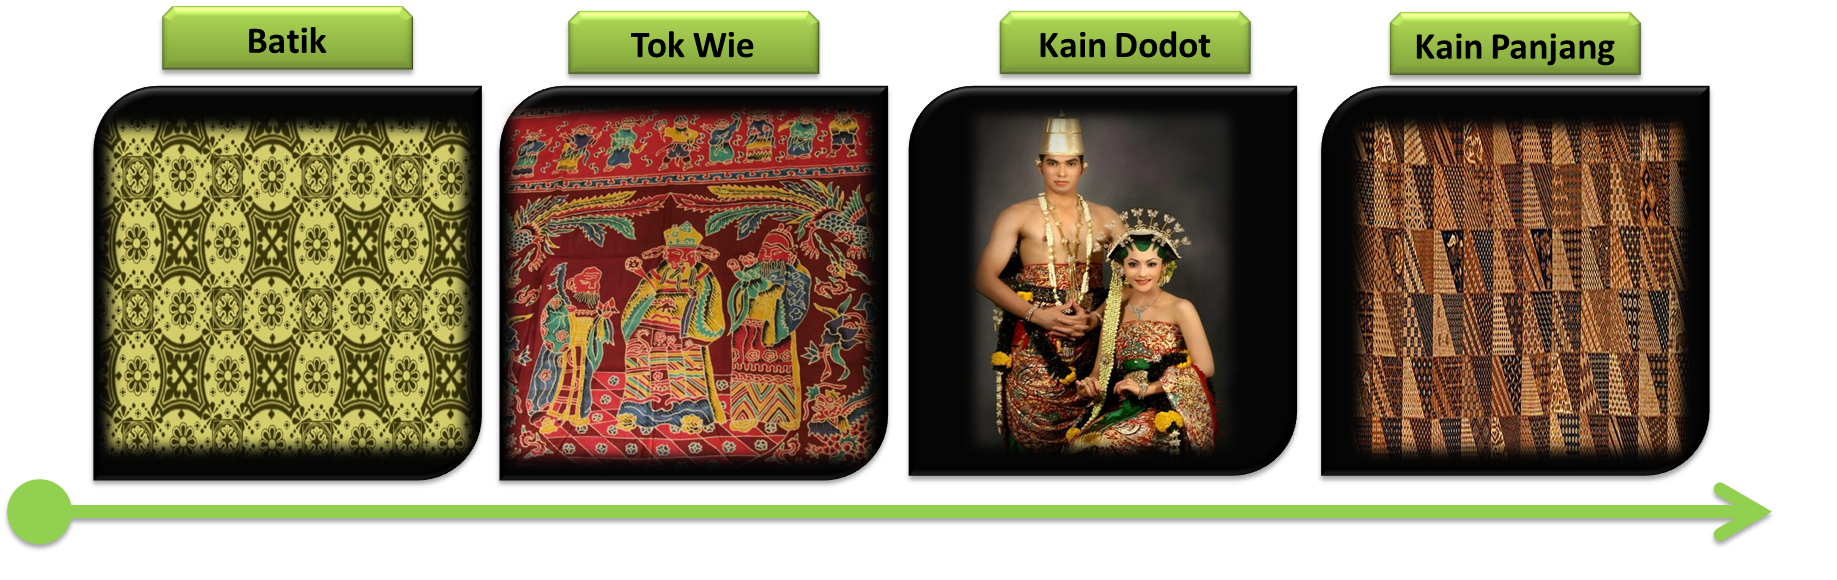
\includegraphics[width=10cm]{pics/kain_indonesia}
	\caption{Contoh kain dari berbagai daerah di indonesia}
	\label{fig:kain_indonesia}
\end{figure}
Salah satu kain tradisional Indonesia adalah batik. Batik merupakan kain bergambar yang memiliki gaya, warna dan tekstur dimana proses pembuatannya dilakukan secara manual maupun menggunakan mesin. Batik memiliki beberapa motif seperti motif kawung, motif parangkusumo, motif truntum, motif tambal, motif pamiluto, motif parang, motif liris maupun motif udan nitik seperti pada gambar \ref{fig:motif_batik}.

Tiap motif batik memiliki makna tersendiri berdasarkan daerah asal batik tersebut. Beberapa makna motif batik (sumber : http://batik-tulis.com/blog/batik-yogyakarta):
\begin{itemize}
	\item Motif ceplok dengan model grompol melambangkan harapan orang tua akan semua hal yang baik terkumpul, yaitu rejeki, kerukunan hidup, kebahagiaan, dan ketentraman untuk kedua mempelai dan keluarga pengantin.
	\item Motif kawung jogja melambangkan segala sesuatu yang bersifat murni, suci, dari putih kembali ke putih.
	\item Motif batik lereng dari yogyakarta melambangkan kesuburan, harapan untuk kemakmuran, tekad, untuk memiliki keberanian untuk melaksanakan apa yang penting bagi bangsa dan rakyat.
	\item Motif nitik dengan "motif cakar ayam biasa dikenakan pada acara perkawinan dengan tujuan agar pasangan yang menikah dapat mencari dengan halal sepandai ayam mencari makan dengan cakarnya".
	\item Motif parang menjadi "pedoman utama untuk menentukan derajat kebangsawanan seseorang dan menjadi pedoman yang termaktub dalam pranatan dalem asmanipun panganggo keprabon wonten kraton nagari ngayogjakarta hadiningrat pada tahun 1927".
\end{itemize} 
\begin{figure}[htp]
	\centering
	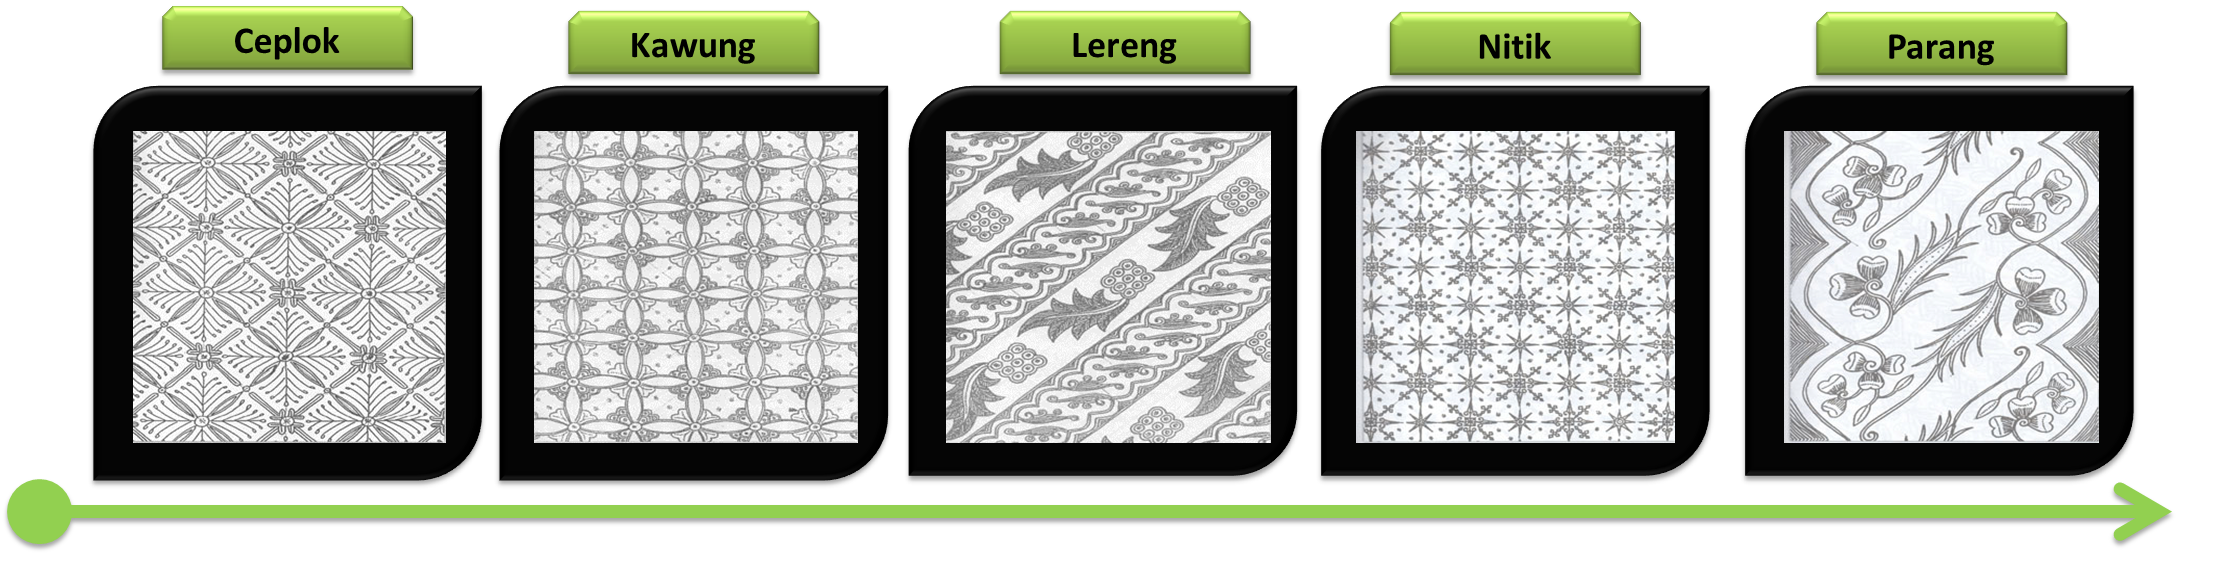
\includegraphics[width=15cm]{pics/motif_batik}
	\caption{Contoh motif batik indonesia}
	\label{fig:motif_batik}
\end{figure}